\documentclass{standalone}

\usepackage[OT1]{fontenc}
\renewcommand*\familydefault{\sfdefault}
\usepackage{helvet,sfmath}
\usepackage{siunitx}

\usepackage{tikz}
\usetikzlibrary{arrows,calc,patterns}
% \usetikzlibrary{intersections, calc, arrows.meta}
\usepackage{tikz,tkz-euclide}

\begin{document}
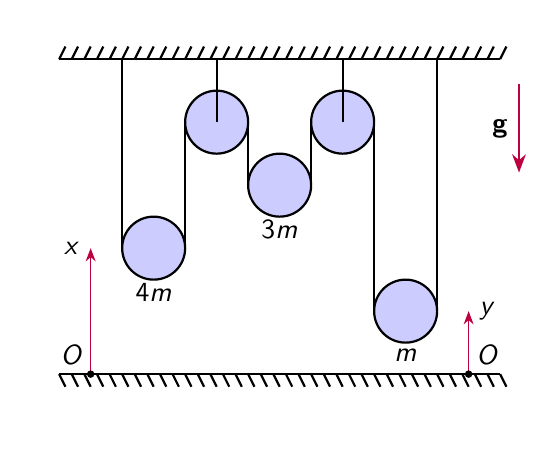
\begin{tikzpicture}[scale=0.8, >=Stealth]

    %% Background
    \draw[draw=none] (-4,-1) rectangle (4,5.5);

    % Pulley
    \draw[thick, fill=blue!20] (-2,2) circle (0.5);
    \draw[thick, fill=blue!20] (0,3) circle (0.5);
    \draw[thick, fill=blue!20] (2,1) circle (0.5);
    \draw[thick, fill=blue!20] (-1,4) circle (0.5);
    \draw[thick, fill=blue!20] (1,4) circle (0.5);

    % Ground
    \draw[thick] (-3.5,5) to (3.5,5);
    \foreach \x in {-3.5,-3.3,...,3.5}
    {
    \draw[thick] (\x,5) to (\x+0.1,5.2);
    }

    % Rope
    \draw[thick] (-2.5,2) to (-2.5,5);
    \draw[thick] (-1.5,2) to (-1.5,4);
    \draw[thick] (-0.5,3) to (-0.5,4);
    \draw[thick] (0.5,3) to (0.5,4);
    \draw[thick] (1.5,1) to (1.5,4);
    \draw[thick] (2.5,1) to (2.5,5);

    \draw[thick] (-1,4) to (-1,5);
    \draw[thick] (1,4) to (1,5);

    % Coordinates
    \draw[purple, -Stealth] (-3,0) to (-3,2);
    \draw[purple, -Stealth] (3,0) to (3,1);
    \draw[fill=black] (-3,0) circle (0.05);
    \draw[fill=black] (3,0) circle (0.05);

    \draw[thick] (-3.5,0) to (3.5,0);
    \foreach \x in {-3.5,-3.3,...,3.5}
    {
    \draw[thick] (\x,0) to (\x+0.1,-0.2);
    }

    \draw
    (-3.3,0.3) node{\(O\)}
    (-3.3,2) node{\(x\)}
    (3.3,0.3) node{\(O\)}
    (3.3,1) node{\(y\)}
    ;

    %Gravity
    \draw[thick, purple, -Stealth] (3.8,4.6) to (3.8,3.2);
    \draw
    (3.5,3.9) node{\(\mathbf{g}\)}
    ;

    % Masses
    \draw
    (-2,1.3) node{\(4m\)}
    (0,2.3) node{\(3m\)}
    (2,0.3) node{\(m\)}
    ;
    
\end{tikzpicture}
\end{document}